\documentclass[a4paper, 10pt]{article}
\usepackage[utf8]{inputenc} % Change according your file encoding
\usepackage{graphicx}
\usepackage{url}

%opening
\title{Seminar Report: Muty}
\date{\normalsize\today{}}

\begin{document}

\maketitle

\begin{center}
  \textbf{Carles Tornel}\\
  \textbf{Jesus Alfaro}\\
  \textbf{Ricard Abril}

\end{center}

\section{Introduction}


\newpage
\section{Experiments}
\paragraph[bold]{Basic Multicast}
\begin{enumerate}
\item Set up the basic multicast system, and use the following test program to experiment with different values for Sleep and Jitter. Sleep stands for up to how many milliseconds the workers should wait until the next message is sent. Jitter stands for up to how many milliseconds the messages are delayed in the network. Duration stands for the duration of the experiment in milliseconds. Note that we are using the name of the multicast module (i.e. basic) as a parameter to the start procedure. We will easily be able to test different multicast implementations. Note also that processes are spawned in different nodes, hence you need to start an Erlang runtime for each process and name it accordingly.\\
\item Make tests with different Sleep and Work parameters to analyze how this lock implementation responds to different contention degrees.
\paragraph[bold]{Test 1: Sleep time major que Jitter time\\\\}
La probabilitat de que un missatge sigui enviat metres estem fent multicast, serà més baixa, ja que és més probable que la resta de nodes es trobin en Sleep time.\\\\
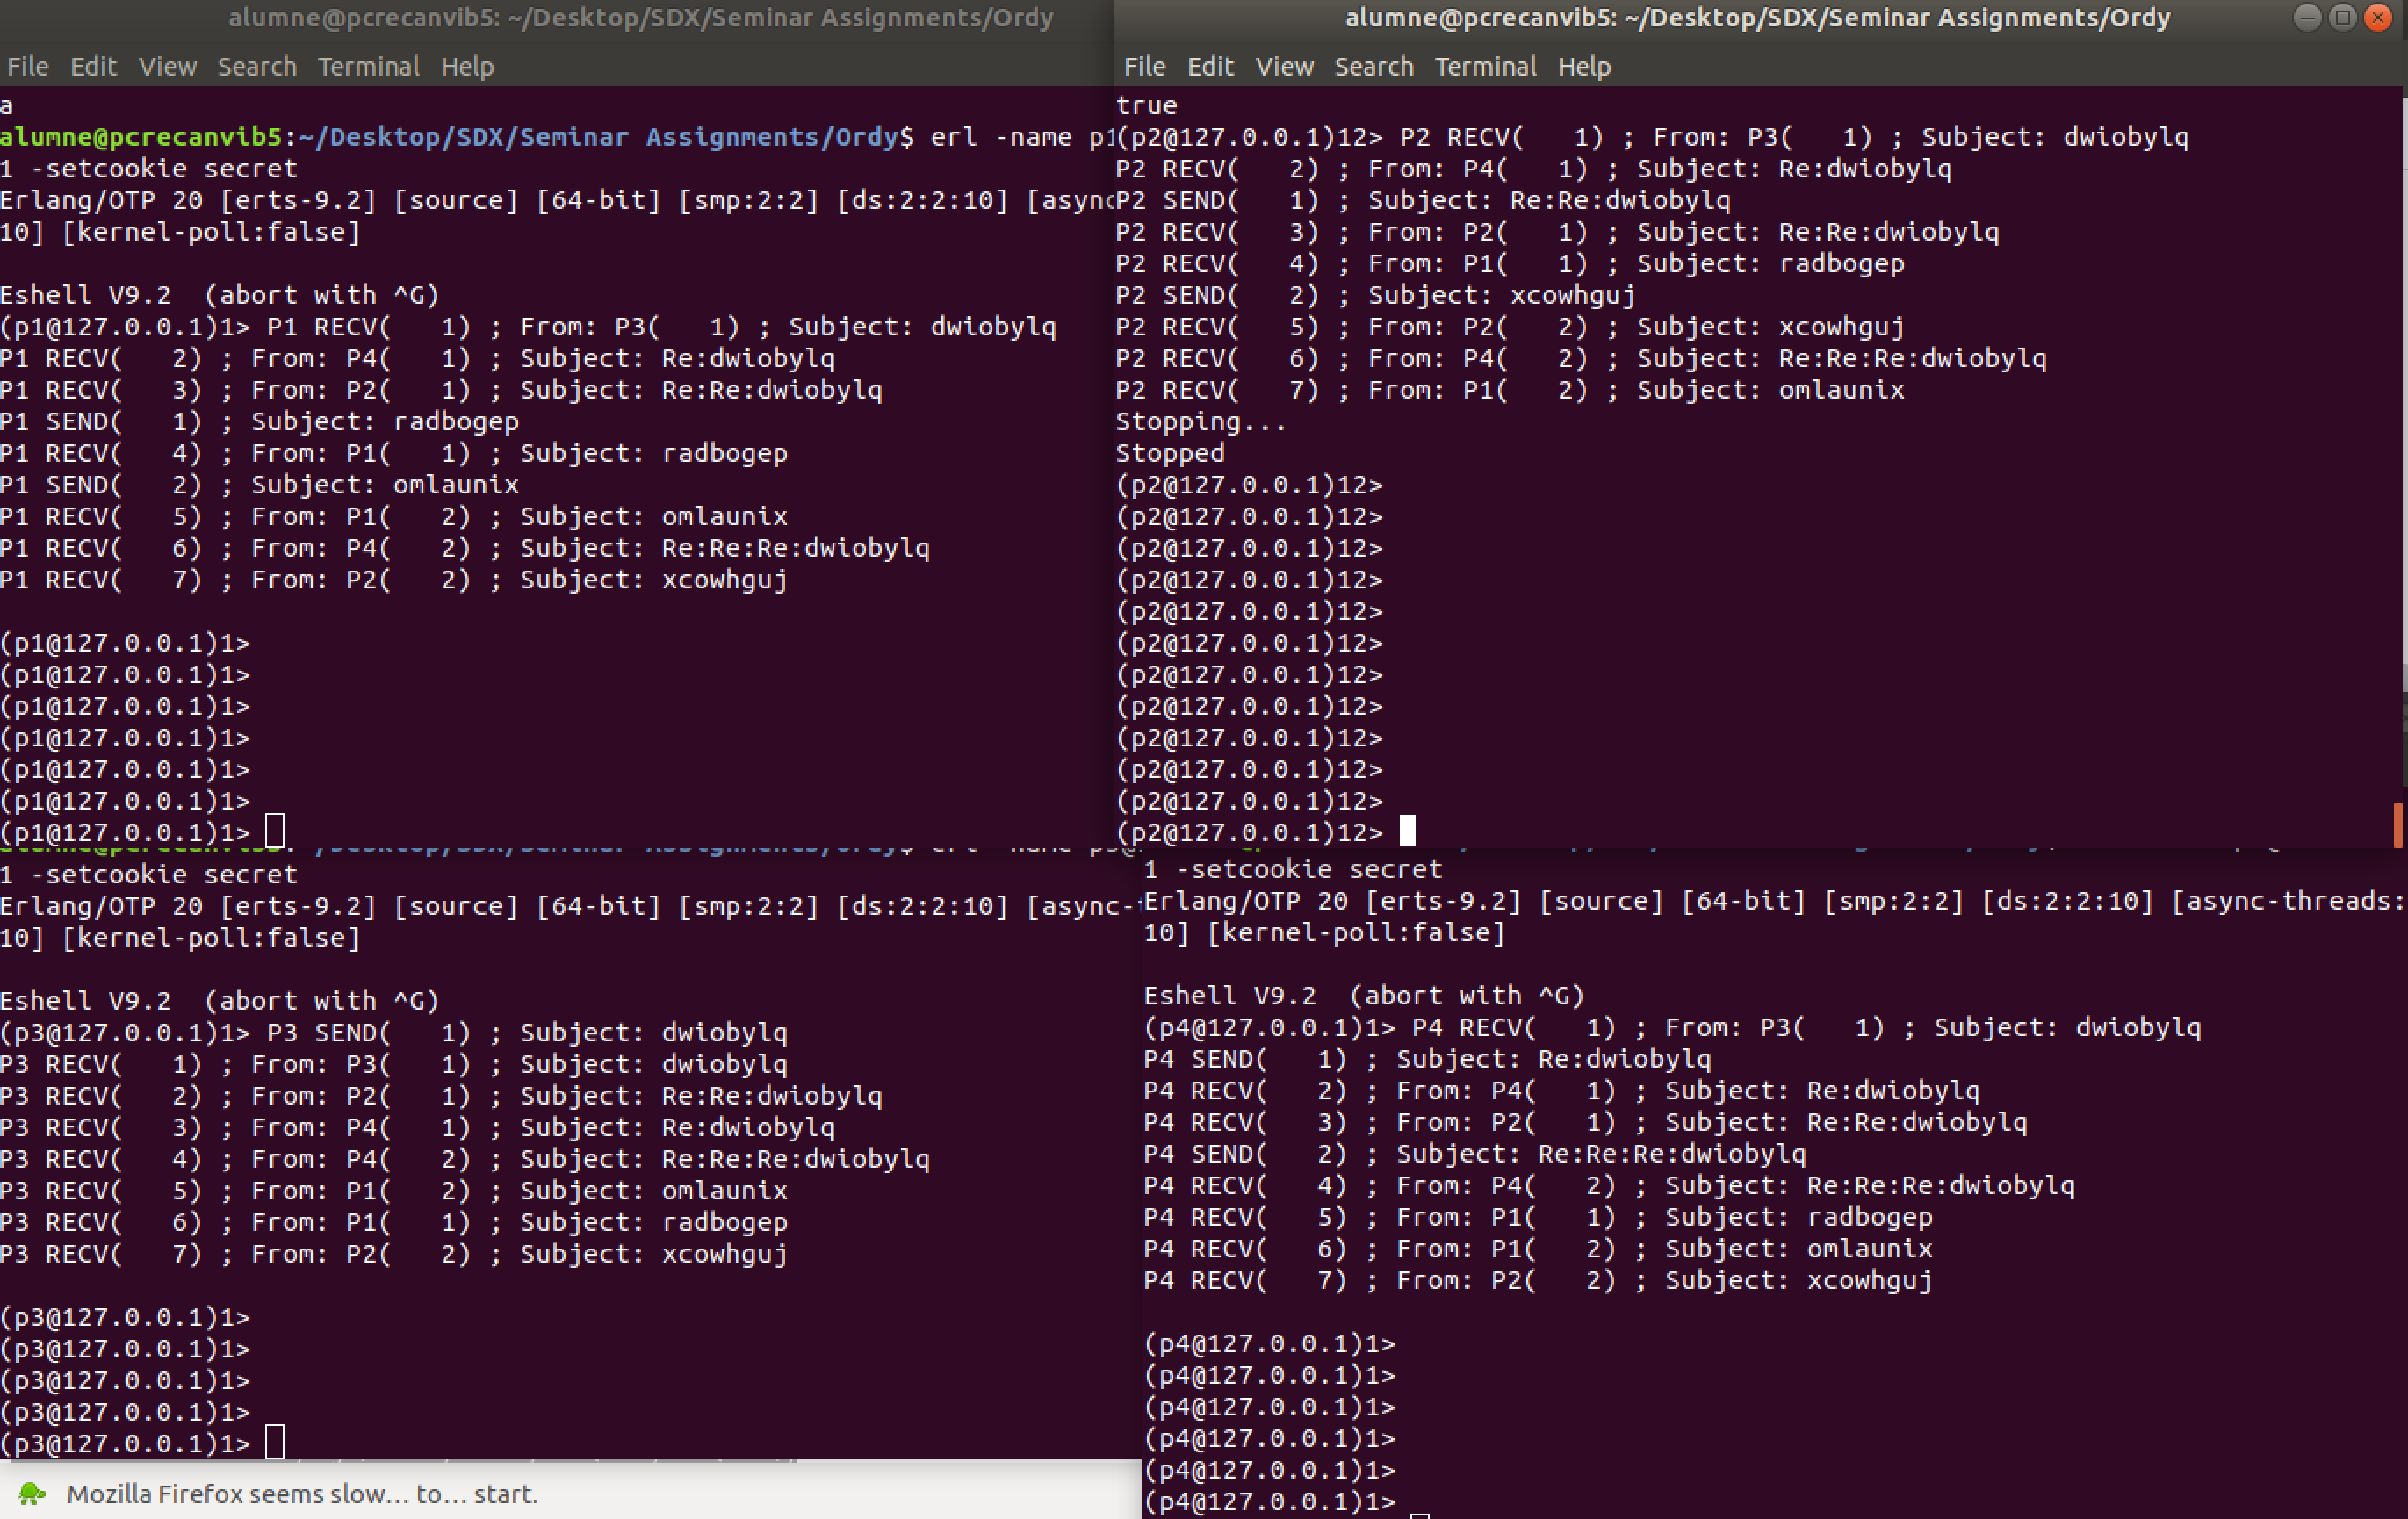
\includegraphics[width=\textwidth]{ordy-basic-1}
\\\\Com podem observar a la figura, hi ha diversos missatges, en el que si que es respecta l'ordre FIFI, però també es pot observar com en alguna ocasió els missatges no arriben en ordre.

\newpage\paragraph[bold]{Test 2: Sleep time inferior a Jitter time\\\\}
En aquet cas, és més probable que l'ordre dels missatges es vegi alterat, ja que en el moment en que estem fent multicast, es més probable que hi hagin missatges a ser enviats, de forma que la probabilitat de que un missatge arribi en desordre és major\\\\
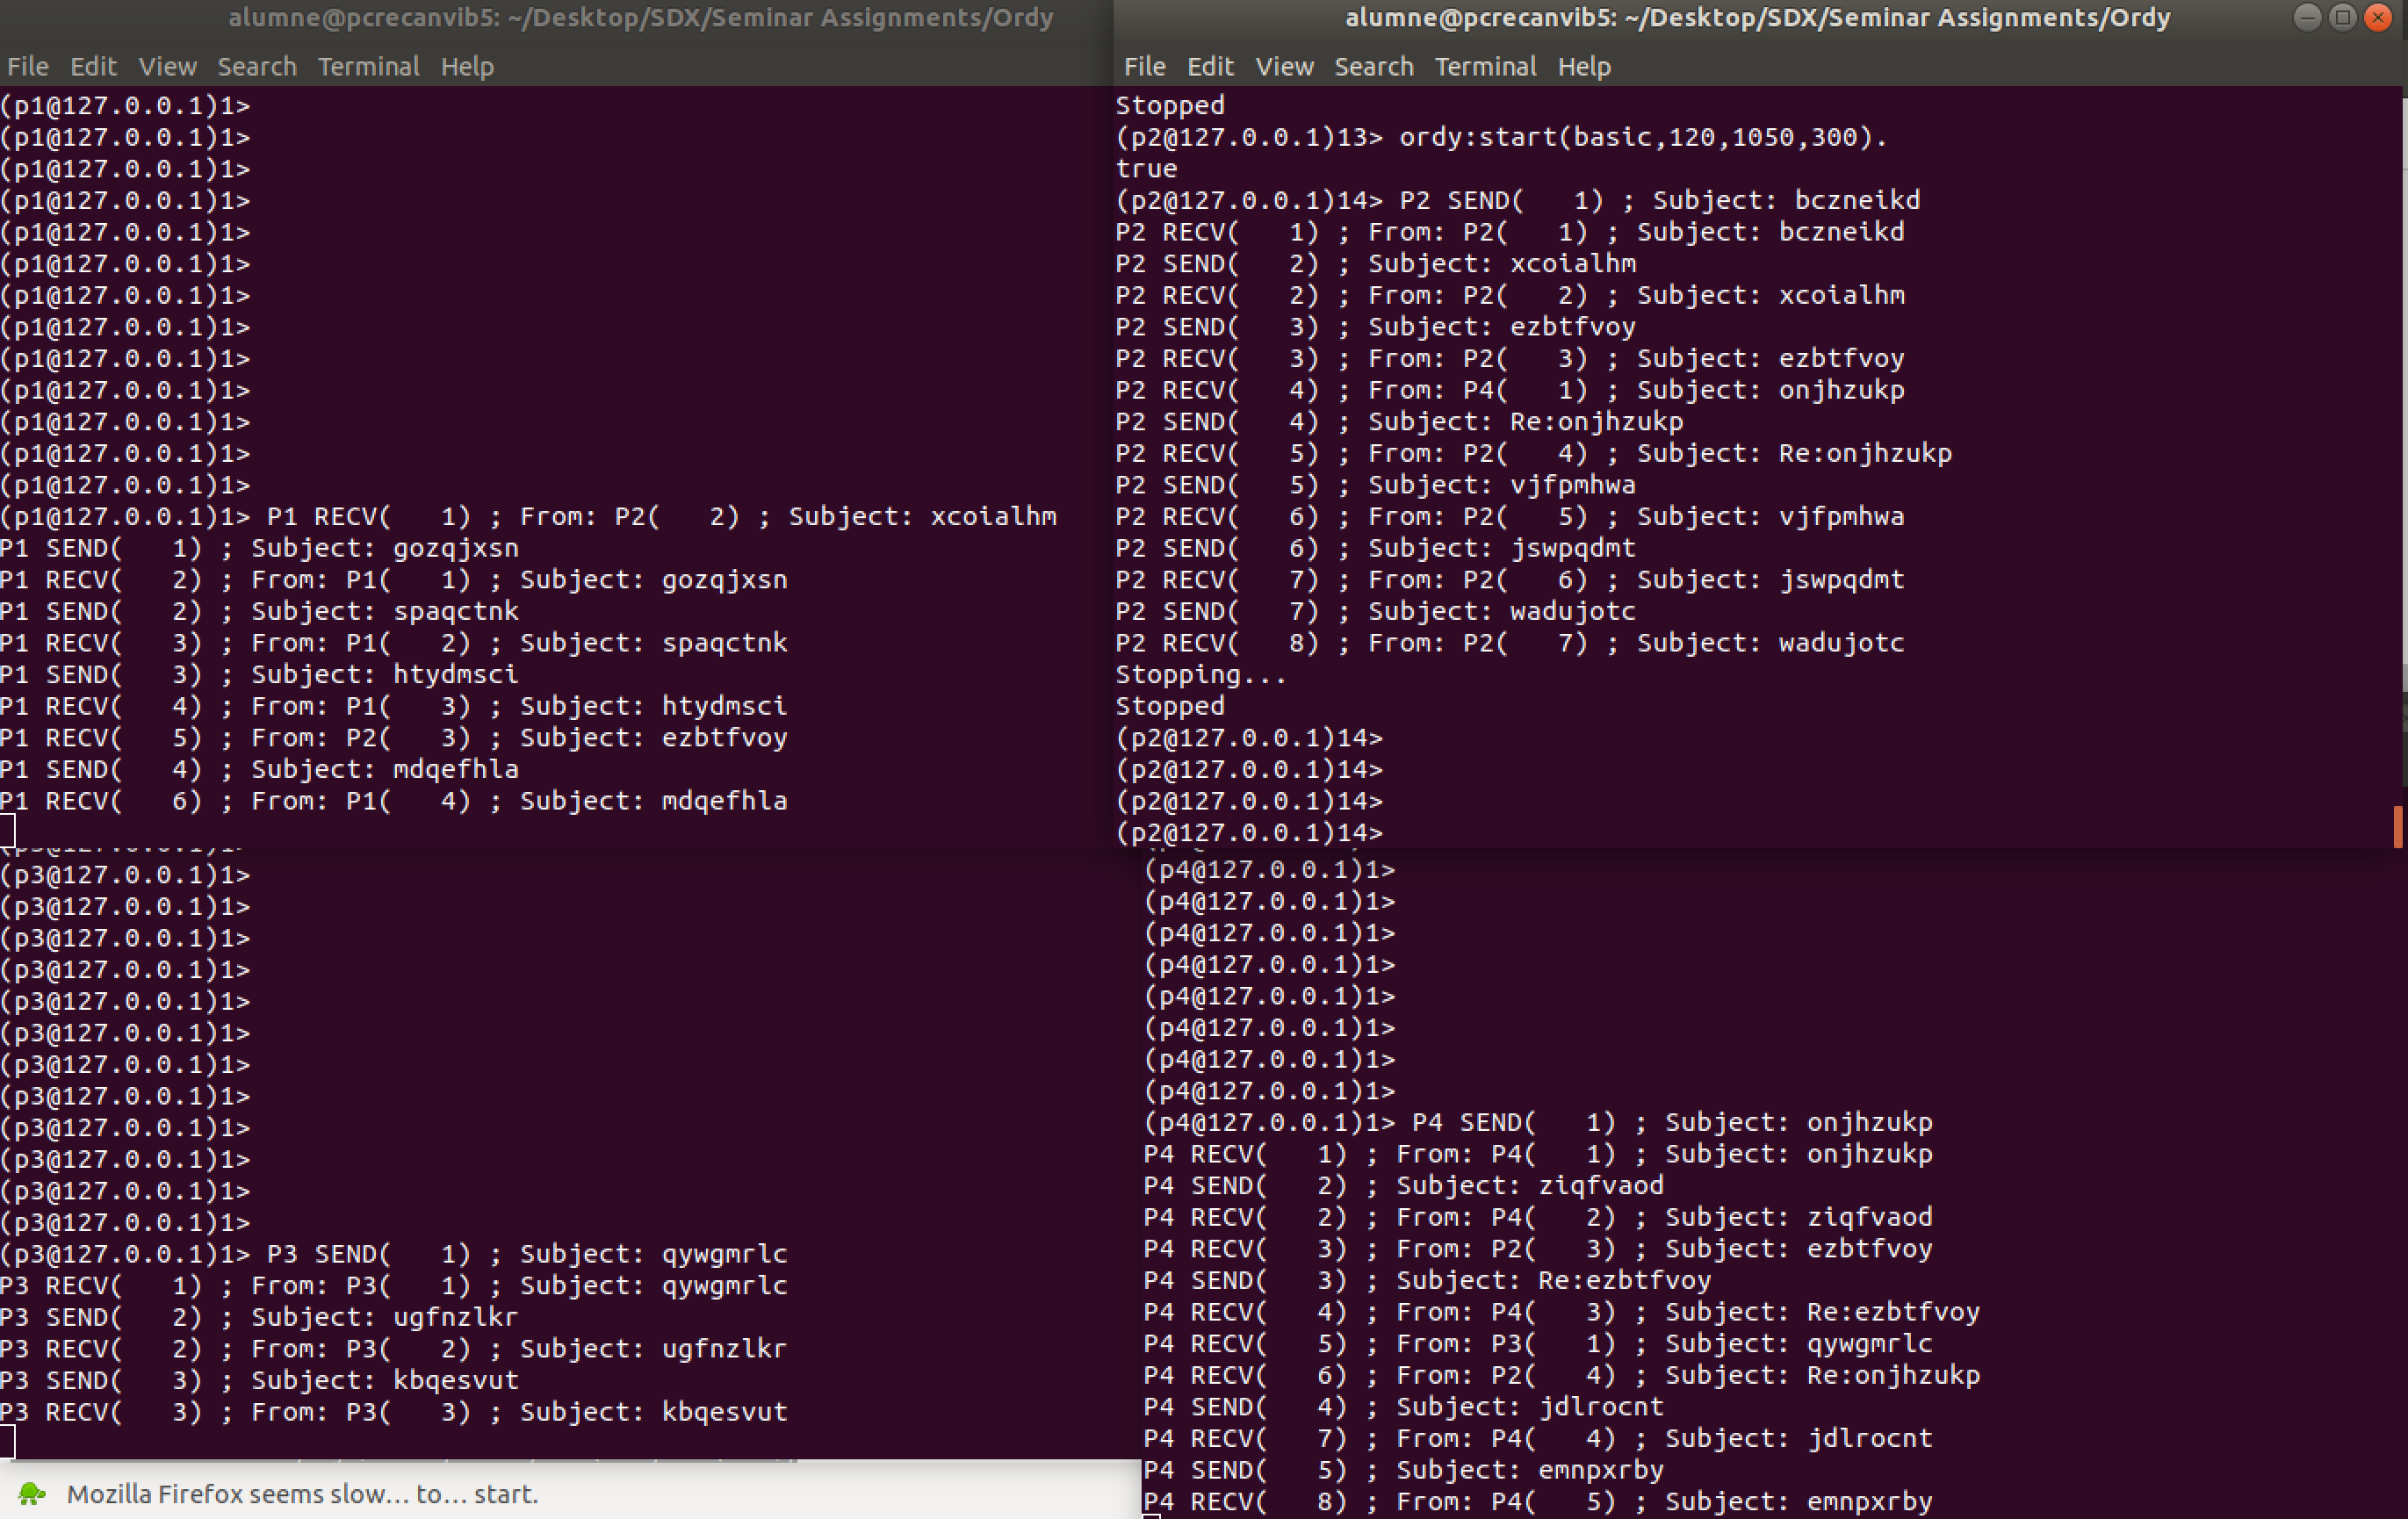
\includegraphics[width=\textwidth]{ordy-basic-2}
\\\\Com podem veure, ara és més fàcil observar desordres en els missatges, degut a que en el període en el que fem multicast, s'estan enviant més missatges.
\end{enumerate}

\newpage
\paragraph[bold]{Causal order multicast}
\begin{enumerate}
\item Set up the causal order multicast system, and repeat the previous tests.\\
\paragraph[bold]{Test 1: Sleep time inferior a Jitter time\\\\}
Amb el Causal order, haurien de arribar els missatges en l'ordre correcte, ja que comprova que el missatge que s’està rebent és el esperat i que s'han rebut tots els anteriors del procés que l'ha enviat.\\\\
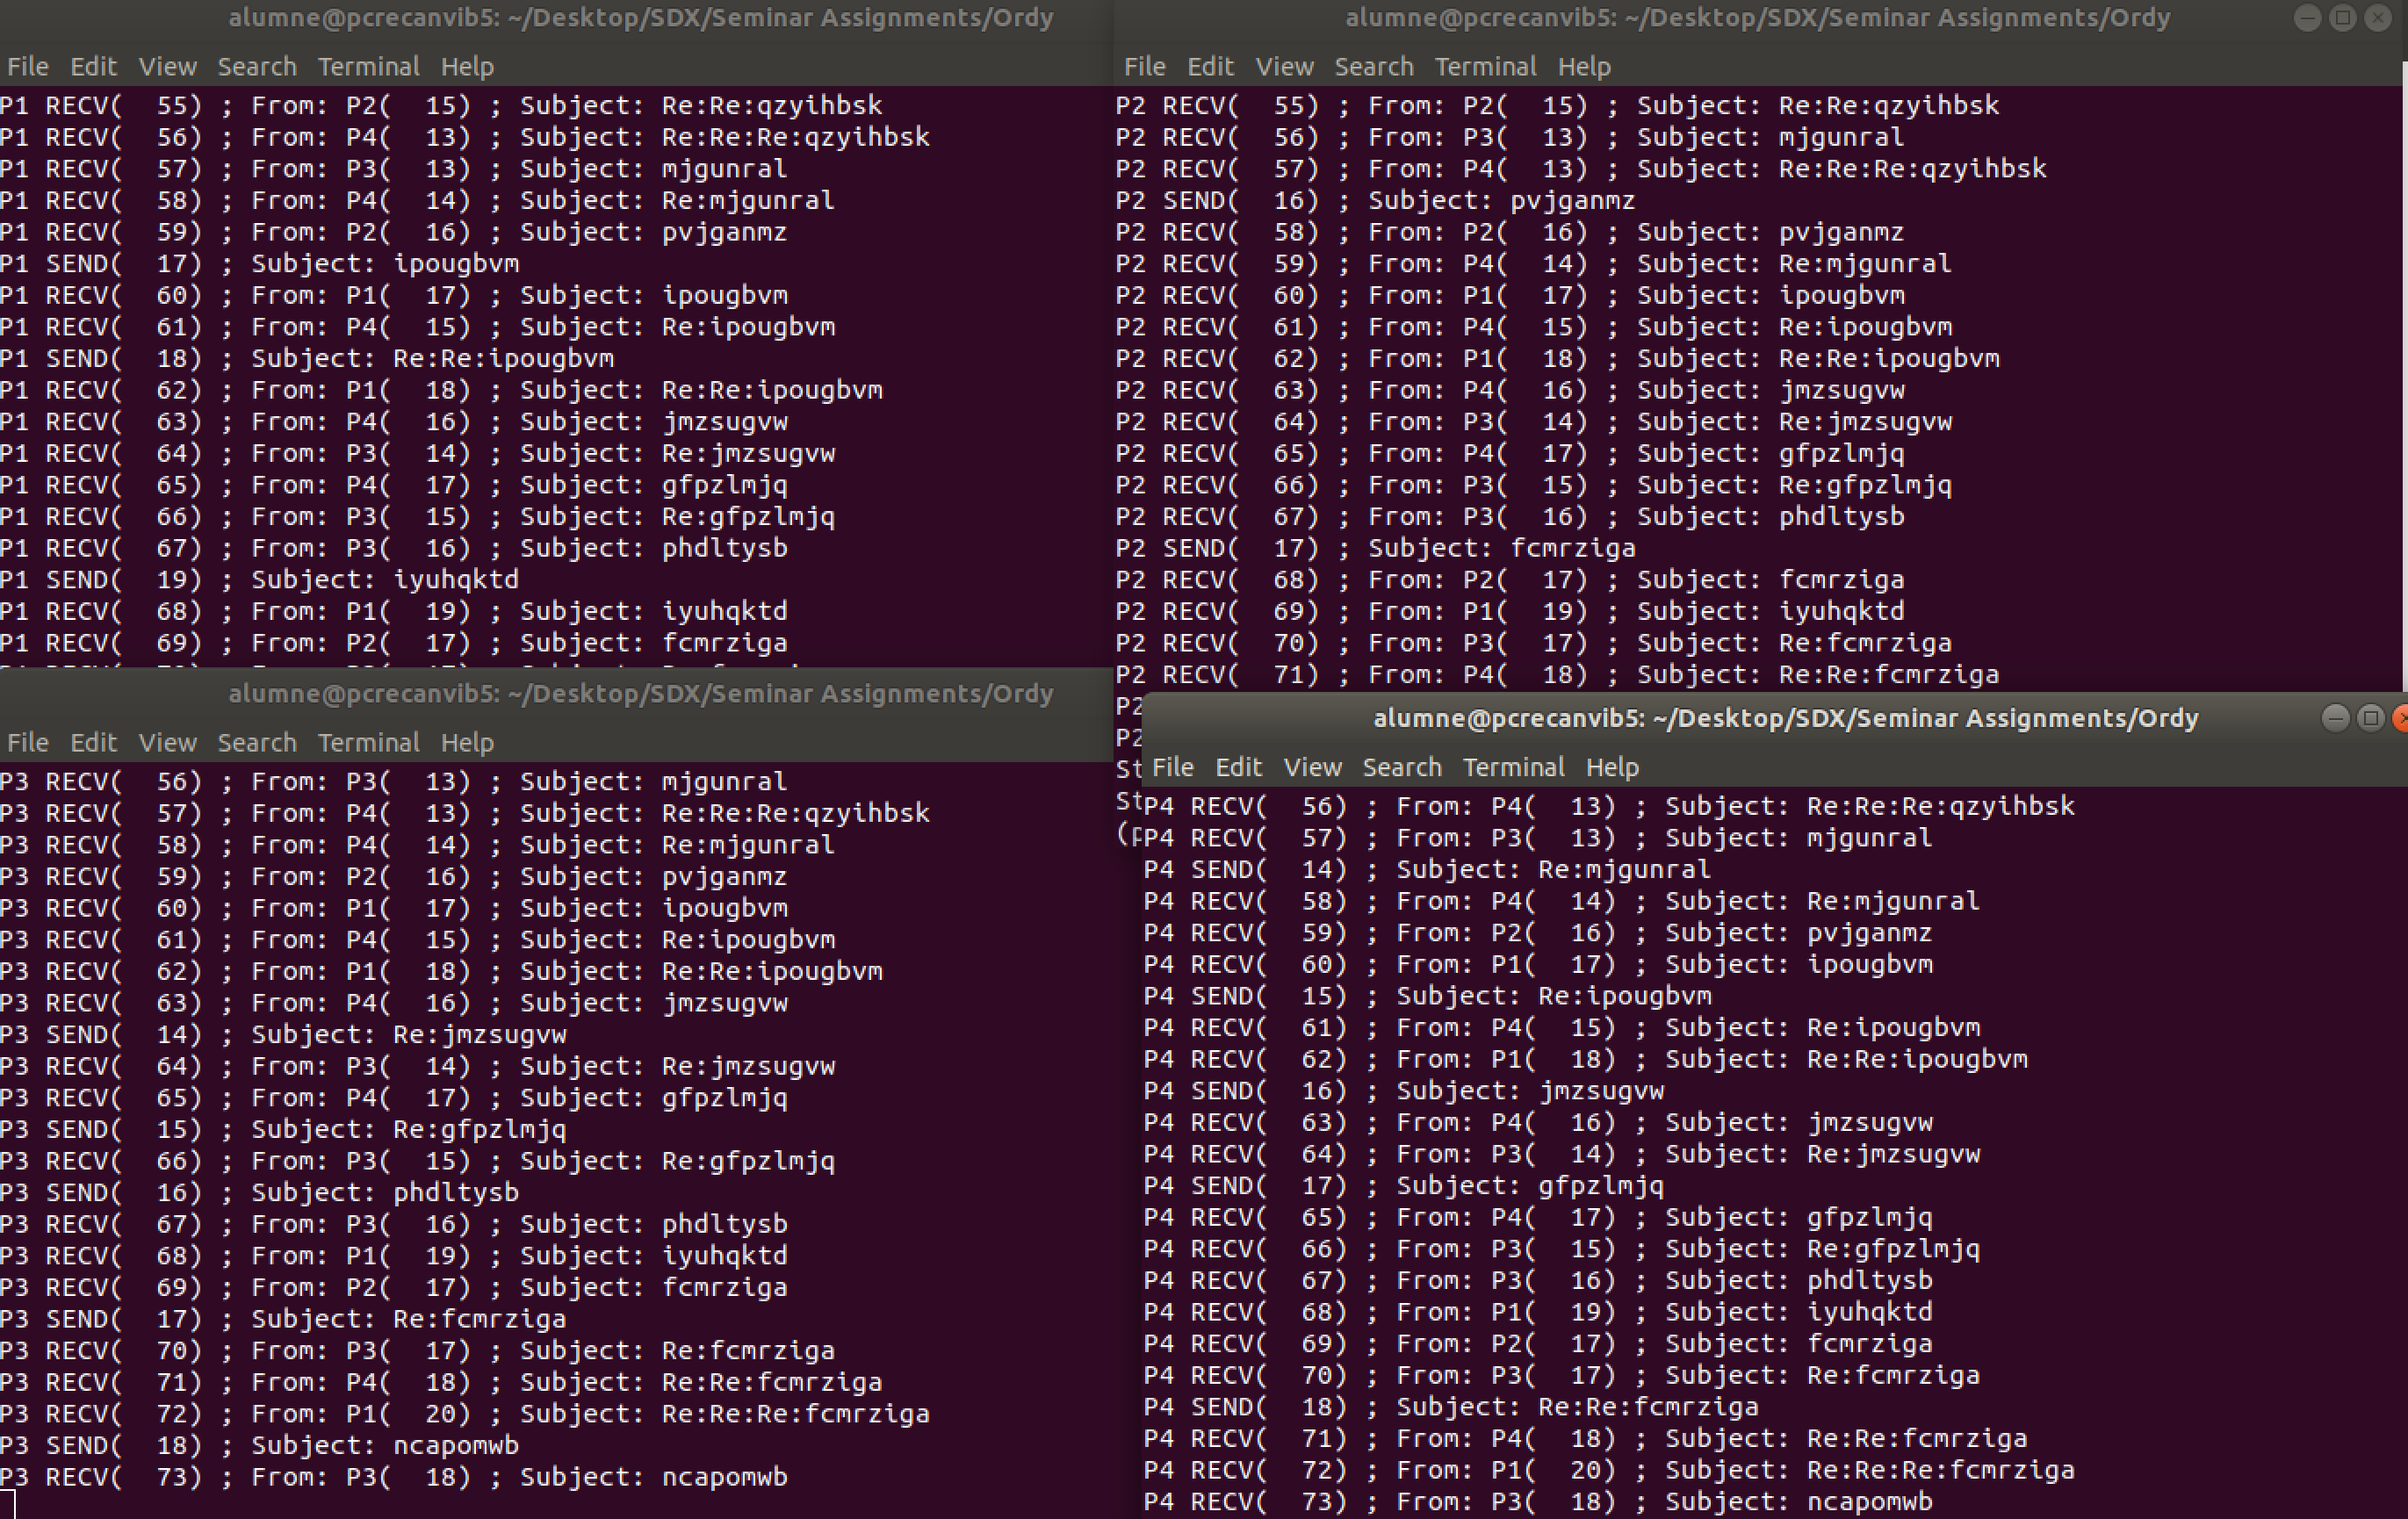
\includegraphics[width=\textwidth]{ordy-causal-1}
\\\\Com podem veure, el ordre s'ha mantes, es a dir no hem rebut ningun missatge no esperat, es a dir que el missatges del emissor arriben en ordre i que no hi ha cap missatge de resposta enviat abans del primer, però el ordre total no s'ha mantes.

\newpage
\paragraph[bold]{Test 2: Sleep time superior a Jitter time\\\\}
El cas de tenir un sleep time menor al Jitter time, no hauria de causar ninguna mena de desordre, en tot cas el que provocarà, és que els missatges triguin més a ser rebuts, ja que els processos estaran en sleep time més estona, com podem veure en la figura.\\\\
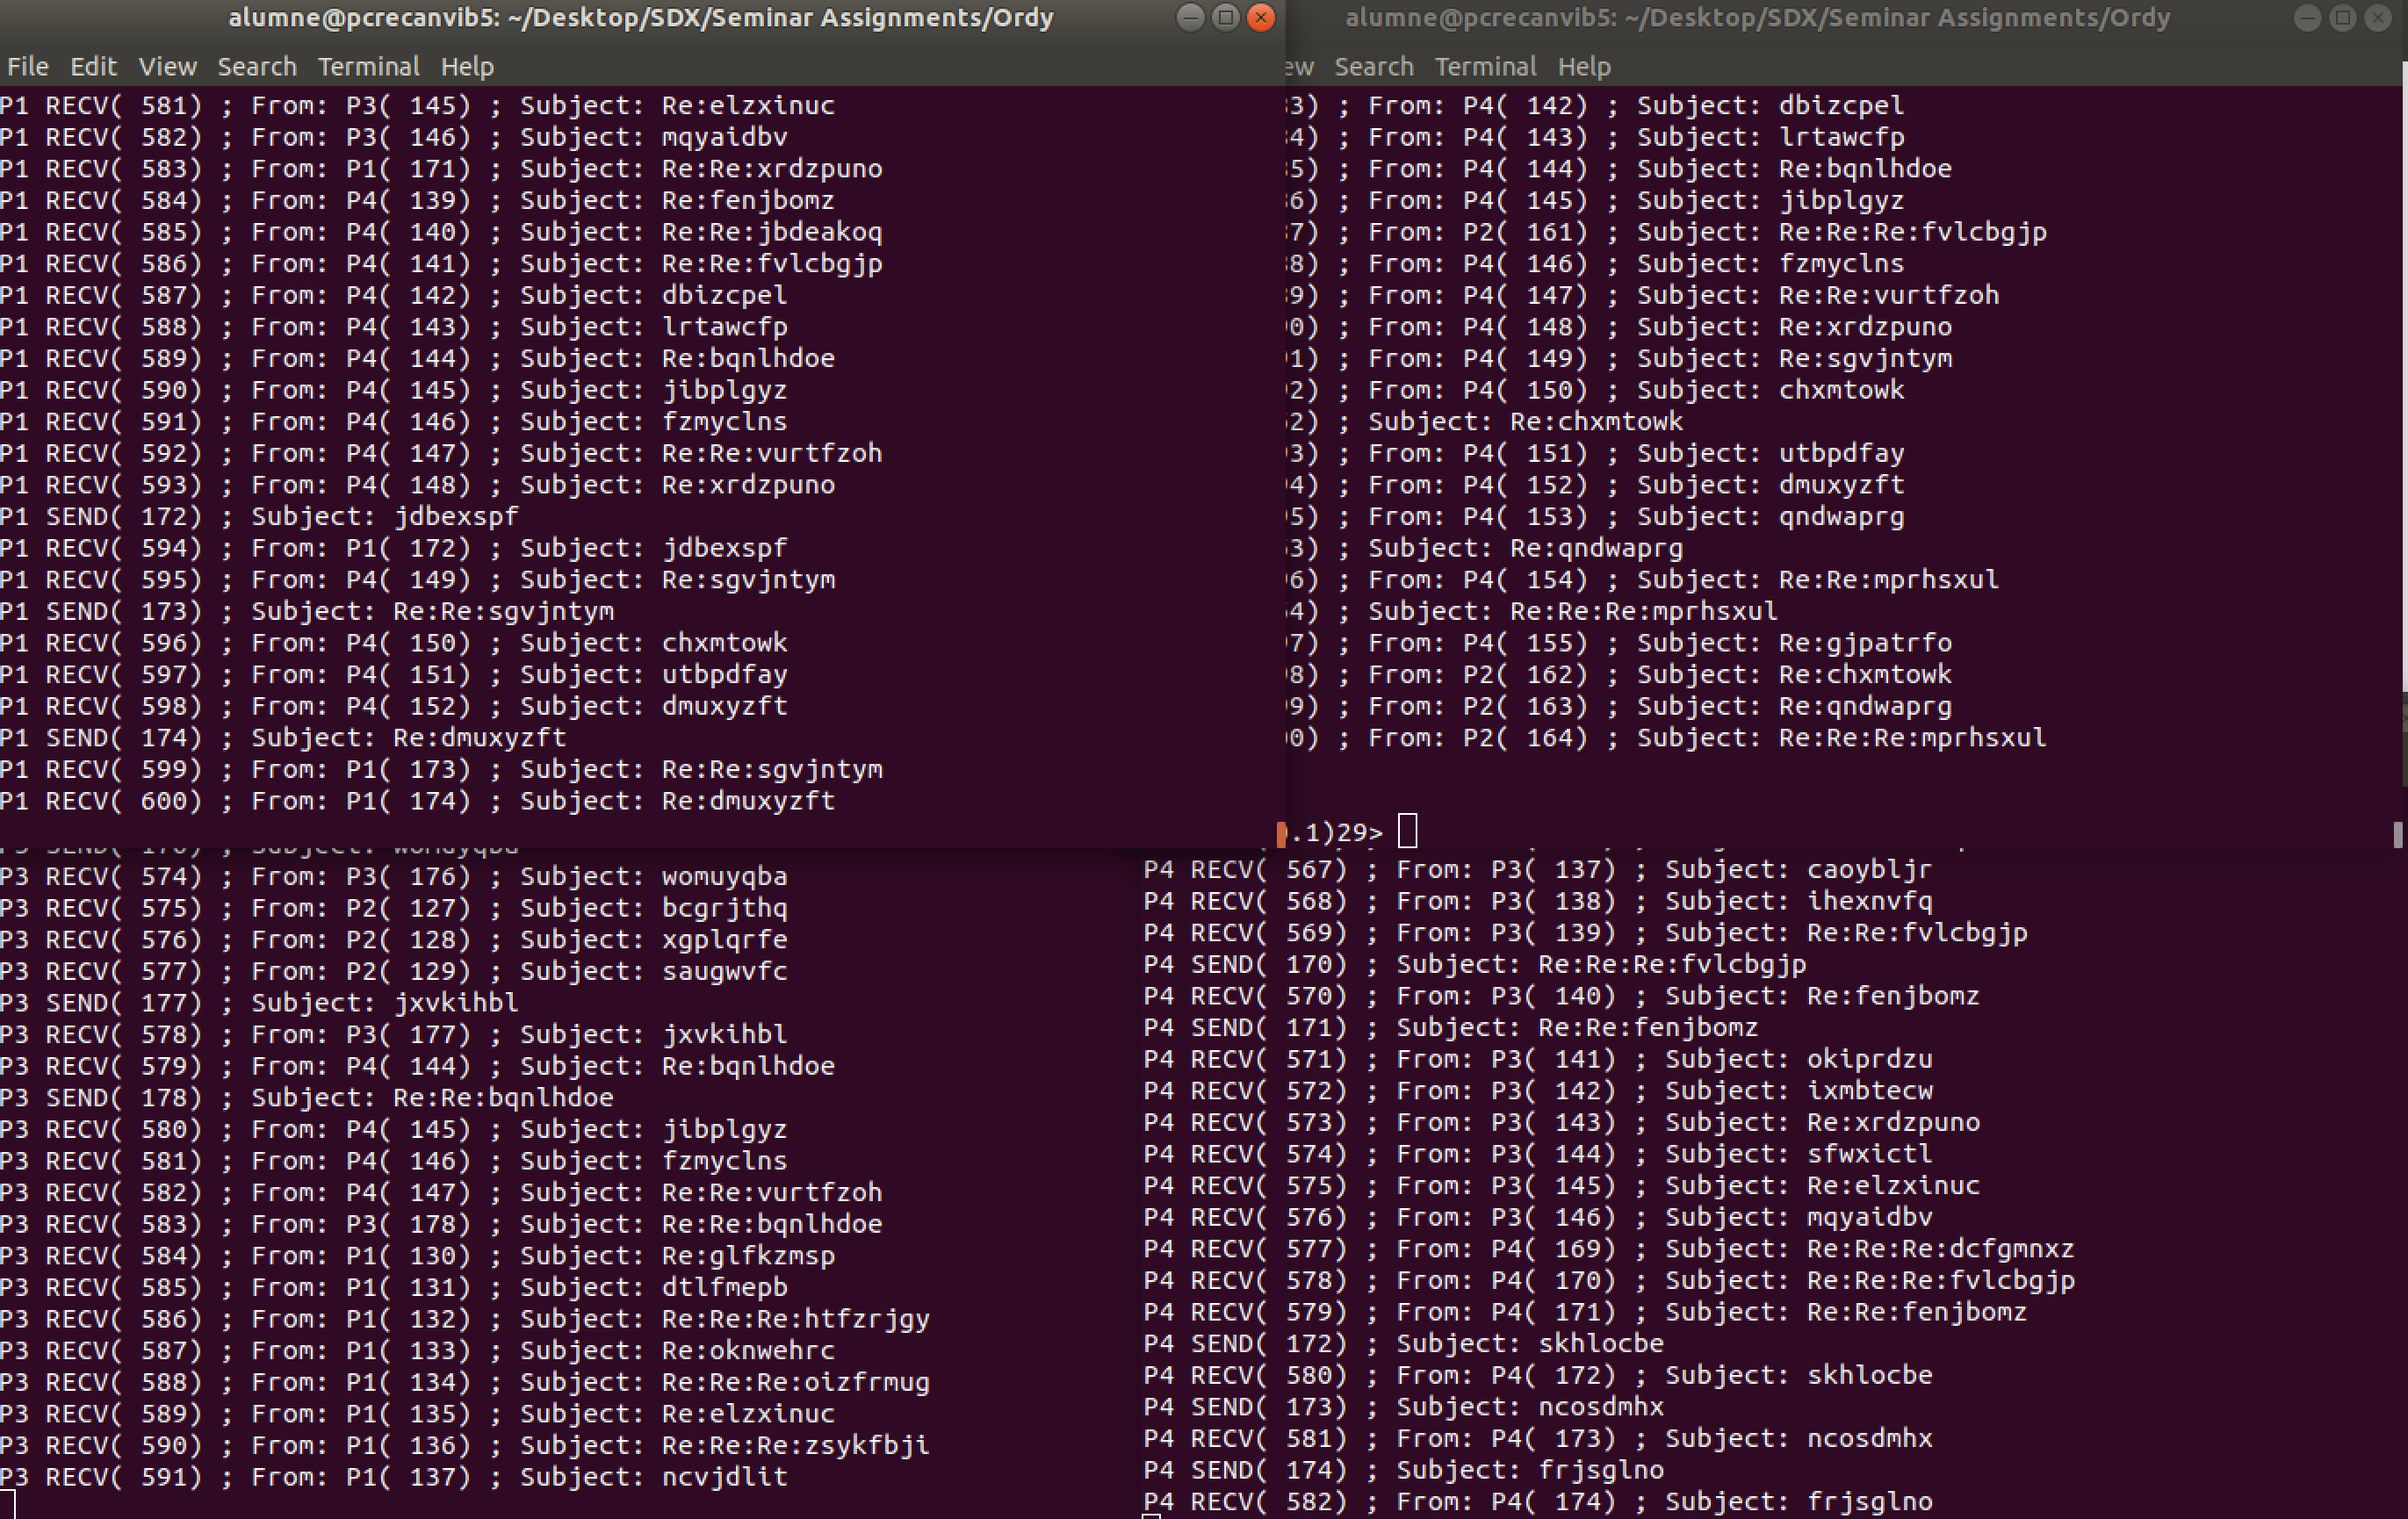
\includegraphics[width=\textwidth]{ordy-causal-2}
\end{enumerate}

\newpage\paragraph[bold]{Total order multicast}
\begin{enumerate}
\item  Set up the total order multicast system, and repeat the previous tests.
\paragraph[bold]{Test 1: Sleep time inferior a Jitter time\\\\}
Ni el Sleep time ni el Jitter time, haurien de provocar cap desordre, ja que els missatges s'entregaran en ordre de mínim nSeq de la queue.\\
El que si que notarem, es que degut al alt temps de Jitter, s'enviaran més missatges.\\\\
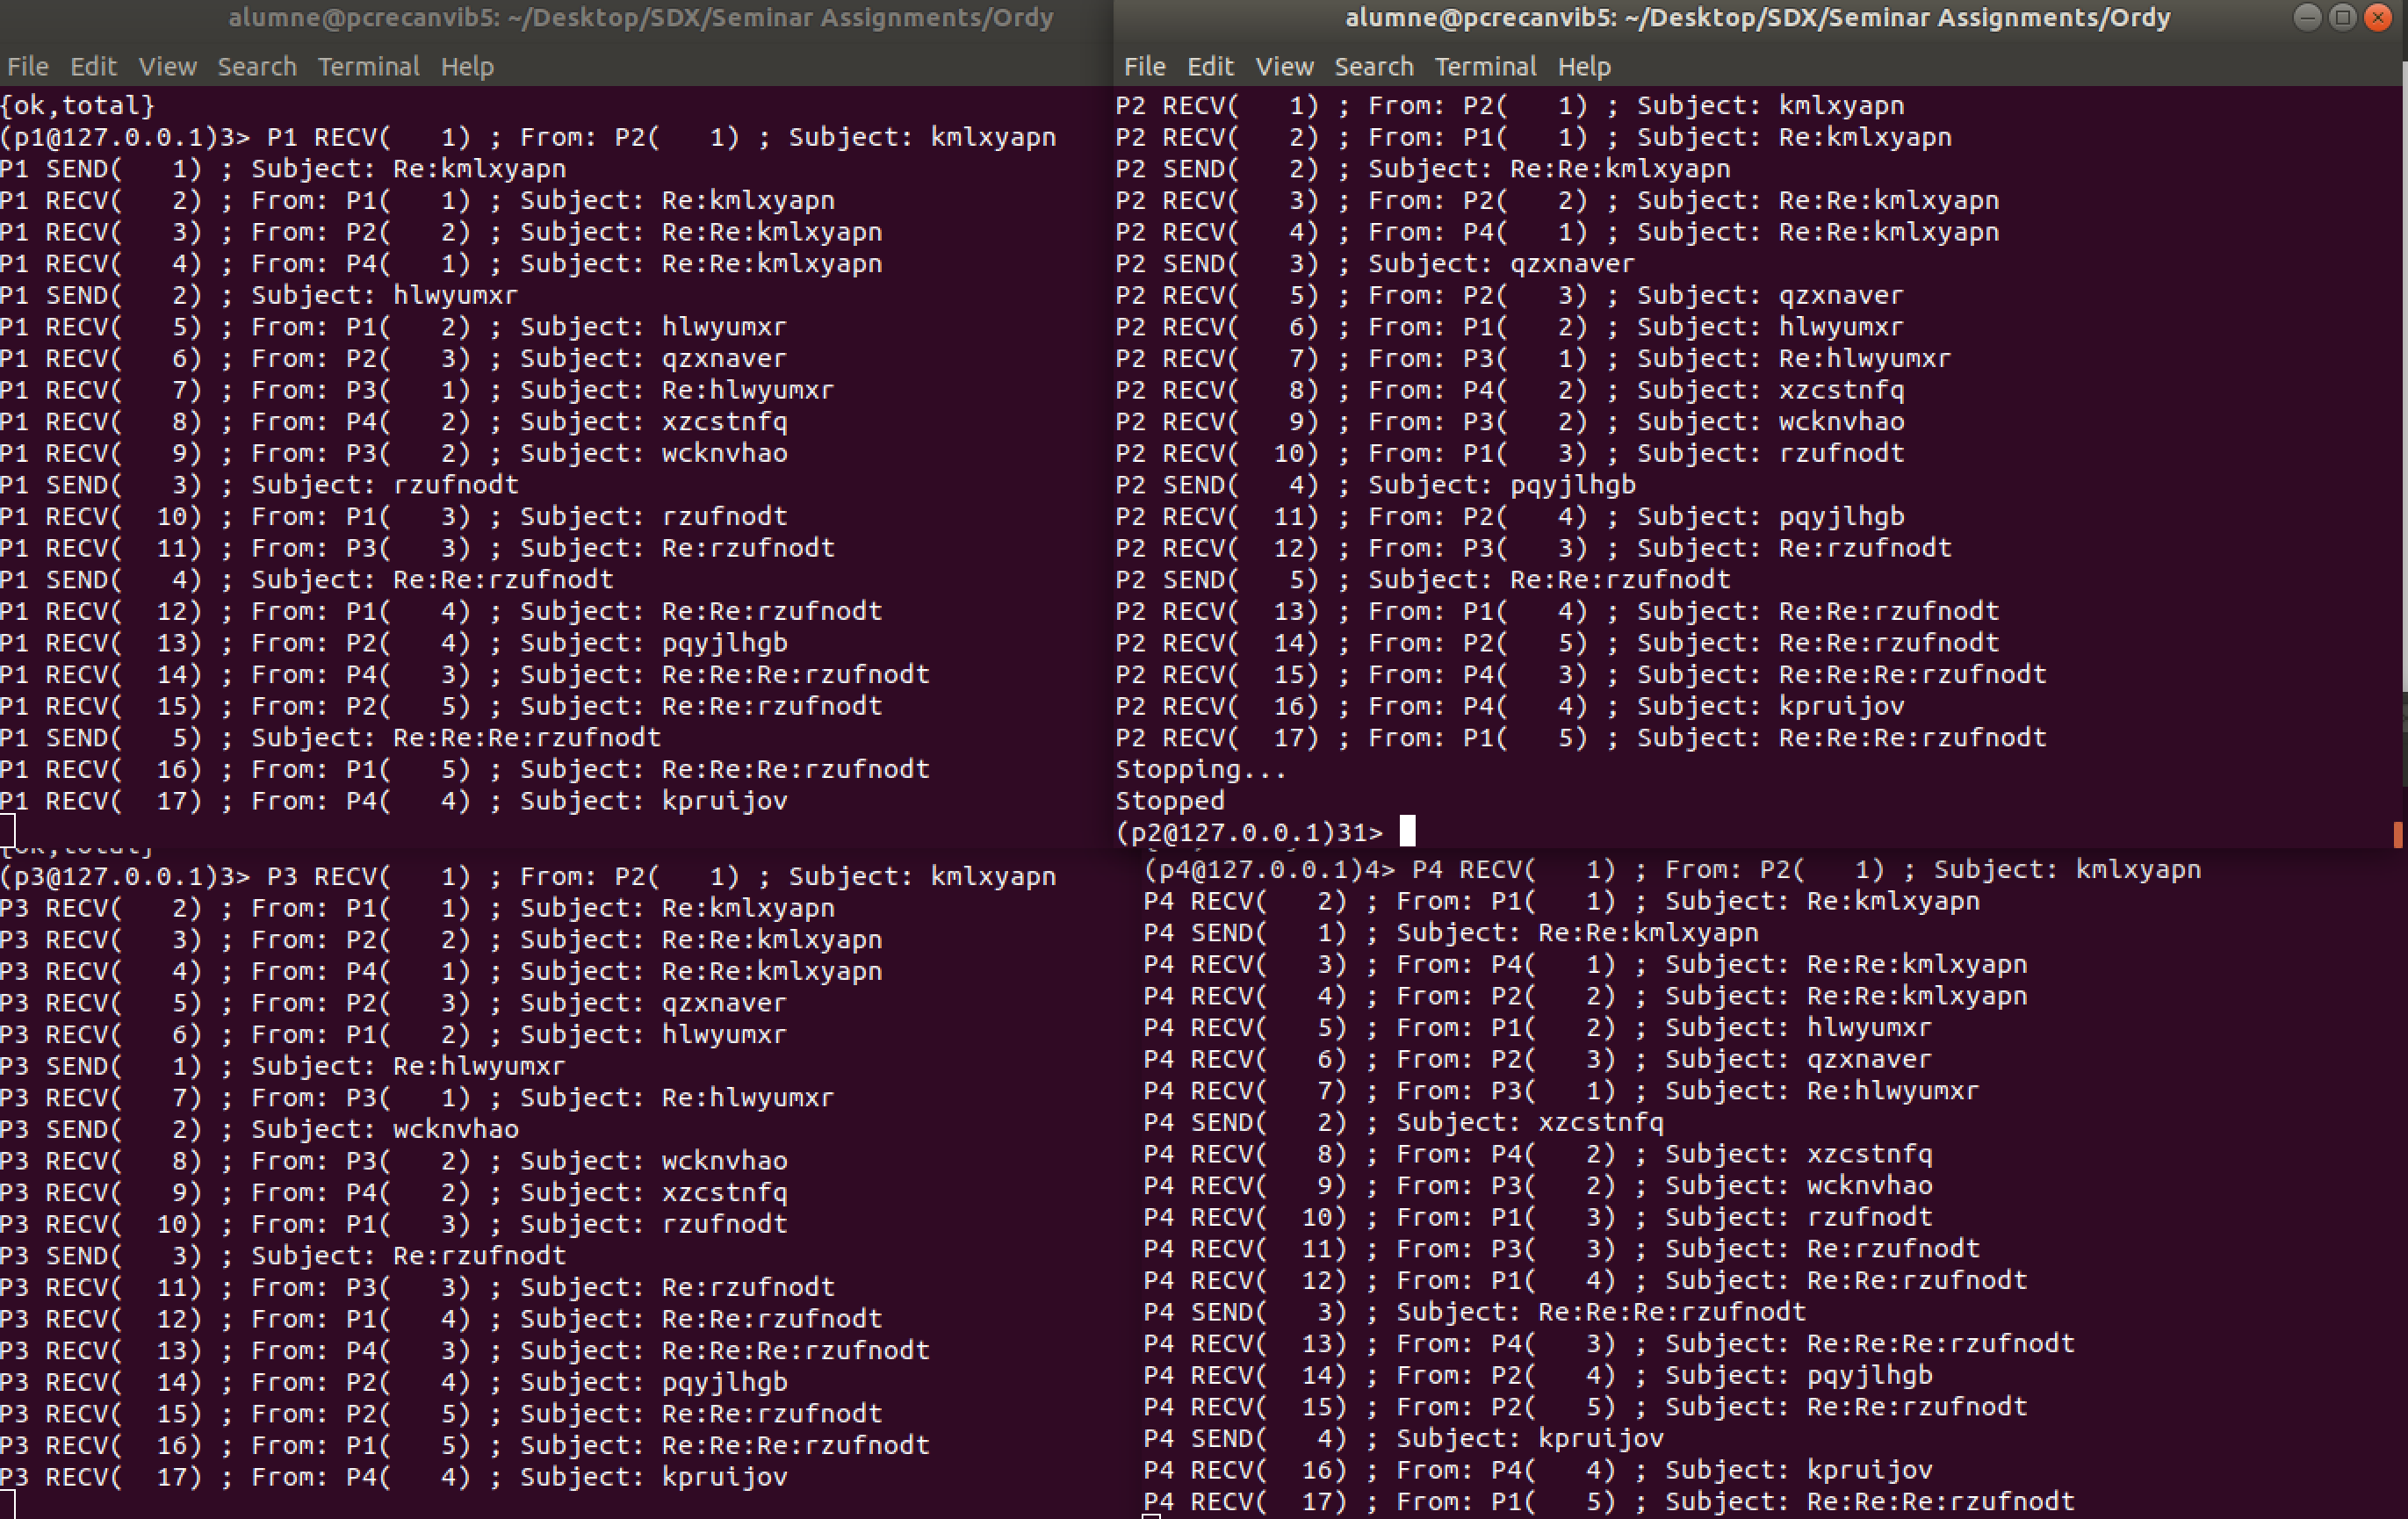
\includegraphics[width=\textwidth]{ordy-total-1}
\newpage\paragraph[bold]{Test 2: Sleep time superior a Jitter time\\\\}
Igual que en el cas anterior, tots els processos rebran els missatges en el mateix ordre, però degut a que el Sleep time, és més alt el numero de missatges rebuts serà menor, tal i com podem veure:\\\\
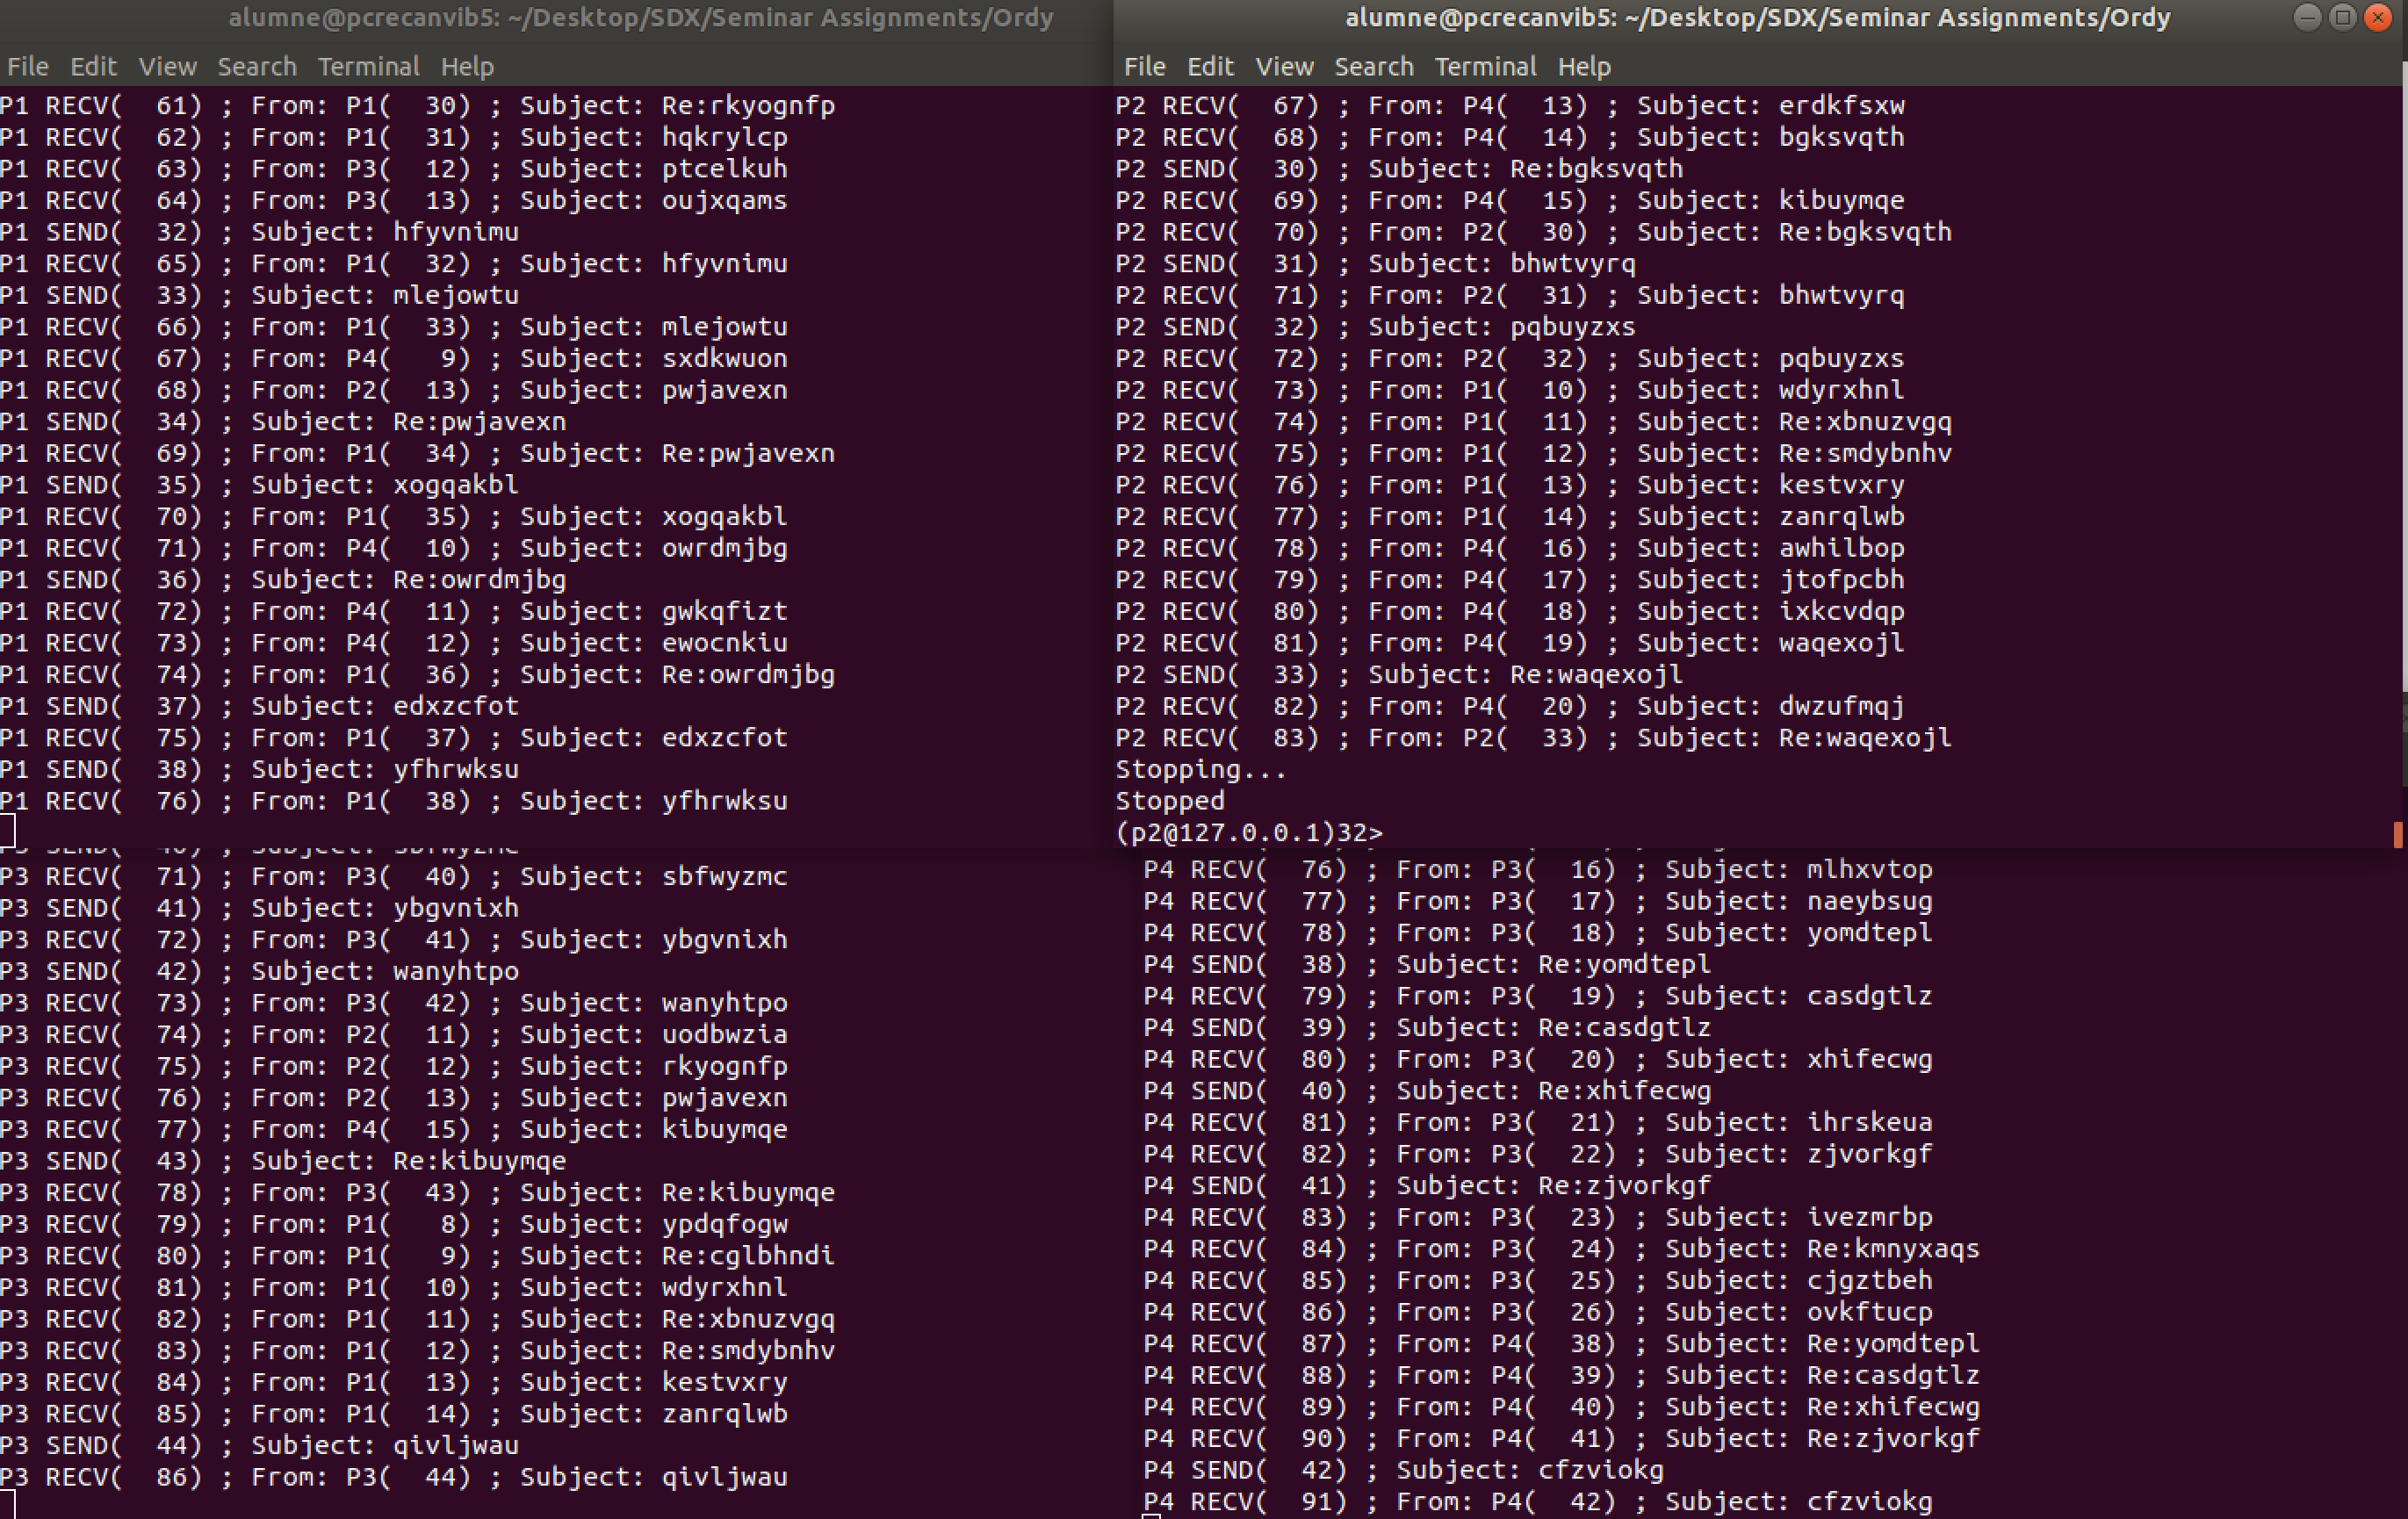
\includegraphics[width=\textwidth]{ordy-total-2}
\\\item We have a lot of messages in the system. Derive a theoretical quantification of the number of messages needed to deliver a multicast message as a function of the number of workers and check exper- imentally that your formulation is correct\\\\
Basic = 1 * send + n * multicast + n * deliver = 2 * n + 1.\\\\
Total = 1 * send + n * request + n * proposal + n * agreed + n * deliver = 4 * n + 1.\\\\
N = numero de workers.

\end{enumerate}

\newpage
\section{Open questions}

\newpage
\section{Personal opinion}
\end{document}
